\question Implement $flower\_keeper$, a function that mutates a tree t so that the only paths that remain are ones which
end in a leaf node with a Tulip flower (‘V’).
For example, consider this tree where only one path ends in a flower. After calling $flower\_keeper$, the tree has
only three nodes left, the ones that lead to the flower:
\newline
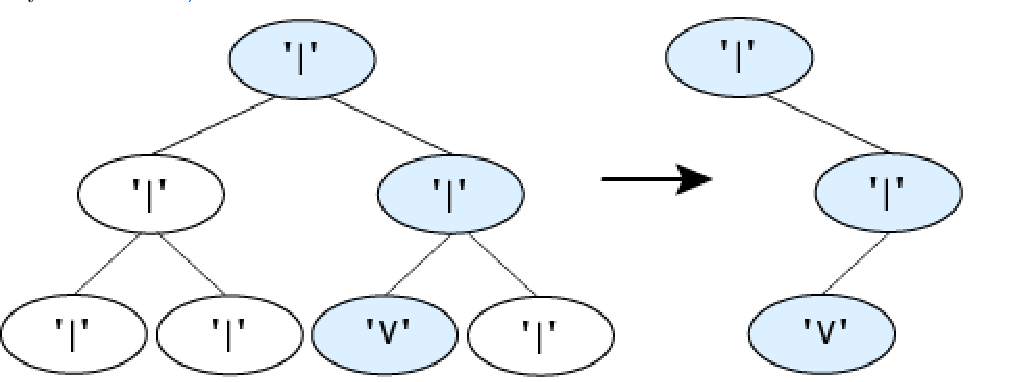
\includegraphics[width=0.8\textwidth]{three-nodes.png}
\newline
\newline

The shaded nodes in the diagram indicate paths that end in flowers.
For this tree where two paths end in flowers, the tree keeps both paths that lead to flowers.
\newline
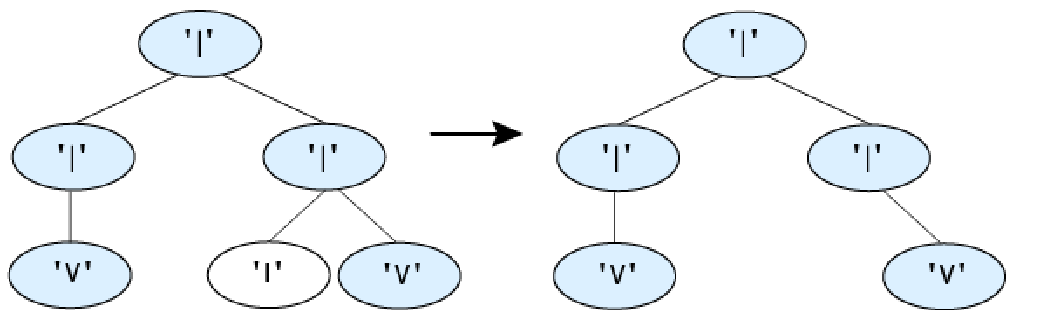
\includegraphics[width=0.8\textwidth]{five-nodes.png}
\newline
\newline

For a tree where none of the nodes are flowers, the function removes every branch except the root node.
\newline
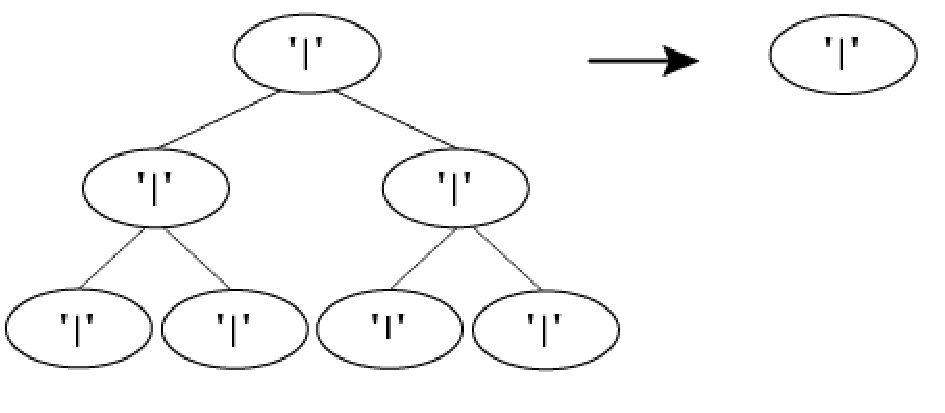
\includegraphics[width=0.8\textwidth]{white-root.png}
\newline
\newline

For a tree with only a single node that is a flower, the function does not remove anything.
\newline
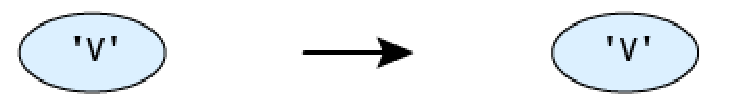
\includegraphics[width=0.8\textwidth]{blue-root.png}
\newline
\newline

\begin{lstlisting}
def flower_keeper(t):
    """
    Mutates the tree T to keep only paths that end in flowers ('V').
    If a path consists entirely of stems ('|'), it must be pruned.
    If T has no paths that end in flowers, the root node is still kept.
    You can assume that a node with a flower will have no branches.
    >>> one_f = Tree('|', [Tree('|', [Tree('|'), Tree('|')]), Tree('|', [Tree('V'), Tree('|')])])
    >>> print(one_f)
    |
        |
            |
            |
        |
            V
            |
    >>> flower_keeper(one_f)
    >>> one_f
    Tree('|', [Tree('|', [Tree('V')])])
    >>> print(one_f)
    |
        |
        V
    >>> no_f = Tree('|', [Tree('|', [Tree('|'), Tree('|')]), Tree('|', [Tree('|'), Tree('|')])])
    >>> flower_keeper(no_f)
    >>> no_f
    Tree('|')
    >>> just_f = Tree('V')
    >>> flower_keeper(just_f)
    >>> just_f
    Tree('V')
    >>> two_f = Tree('|', [Tree('|', [Tree('V')]), Tree('|', [Tree('|'), Tree('V')])])
    >>> flower_keeper(two_f)
    >>> two_f
    Tree('|', [Tree('|', [Tree('V')]), Tree('|', [Tree('V')])])
    """
    for b in __________:

        __________

    __________ = [__________ for b in __________ if __________]
\end{lstlisting}
\begin{solution}[0.5in]
\begin{lstlisting}
    for b in t.branches:
        flower_keeper(b)
    t.branches = [b for b in t.branches if b.label == 'V' or not b.is_leaf()]
\end{lstlisting}
\end{solution}
